% Provenance (never printed): see sources/outline_sources.md (Year 2: natural hazards and risks
% quantified --- recurrence, probabilistic hazard, slope stability, tsunamis, floods, warning).
% Terminology from the UN report A/71/644 (UNDRR); the 475-year convention from the USGS
% Earthquake Hazards 201 page; the ground-motion prediction equation of Boore, Joyner and Fumal
% (USGS Open-File Report 93-509); run-ups from the NOAA NCEI tsunami database; the 1999 Vargas
% debris flows from USGS Open-File Report 01-0144. Ledger rows in sources/ledger/book4.md;
% curves and numbers from figdata/bachelor-2/hazards.py and the Book 4 second-writer scratch
% calculator calc/ch28.py. Hazards are described and quantified physically only: no advice.
\chapter{Geologische gevaren en risico}\label{ch:b2:geological-hazards}

Een gebouw dat ontworpen is voor de grondbeweging die gemiddeld eens in 475 jaar wordt overschreden, heeft een
kans van één op tien om die tijdens een levensduur van vijftig jaar te ondergaan. De twee uitspraken zijn hetzelfde getal,
op twee manieren gelezen, en het heen en weer gaan tussen beide is het dagelijkse werk van de gevarenwetenschap. Dit hoofdstuk
bouwt haar instrumenten op: de kans op zeldzame gebeurtenissen, de \omterm{def:b2:geological-hazards:psha}{gevarencurve} van een locatie, de stabiliteit van een
helling, de snelheid en de \omterm{def:b2:geological-hazards:tsunami}{oploophoogte} van een tsunami, de frequentie van overstromingen, en de fysica die bepaalt
hoeveel waarschuwingstijd elk gevaar kan geven.
% ledger: usgs:eh201-475

\begin{recall}
\textbf{Uit de schoolboeken}: natuurgevaar, natuurramp en aardverschuiving; kwetsbaarheid,
risico, preventie en de gevarenkaart; tsunami; de \omterm{def:b2:geological-hazards:return}{terugkeerperiode} van een overstroming, en de rangformule
$T = (n + 1)/m$ voor een reeks van $n$ jaarlijkse pieken. \textbf{Uit Boek~3}: de
wet van Gutenberg--Richter $\log_{10} N(\geq M) = a - bM$ en haar b-waarde; seismisch moment en
momentmagnitude; poriëndruk, effectieve spanning $\sigma' = \sigma - u$ en het
bezwijkcriterium van Coulomb $\tau = c' + \sigma' \tan\varphi'$. \textbf{Uit \cref{ch:b2:eruptive-styles}}: \omterm{def:b2:eruptive-styles:pdc}{pyroclastische
dichtheidsstromen}, \omterm{def:b2:eruptive-styles:lahar}{lahars} en tefraneerslag. \textbf{Uit de wiskundeboeken}: de poisson- en
exponentiële verdeling, de normale verdeling en haar verdelingsfunctie $\Phi$.
\textbf{Uit het natuurkundeboek van het tweede jaar universiteit}: de dispersierelatie van oppervlaktegolven onder invloed van de zwaartekracht,
$\omega^2 = gk\tanh(kh)$.
\end{recall}

\section{Gevaar, blootstelling en risico}\label{sec:b2:geological-hazards:risk}

\begin{definition}[Geologisch gevaar, blootstelling, rampenrisico]\label{def:b2:geological-hazards:risk}
Een \emph{geologisch gevaar}\index{geologisch gevaar} is een proces of verschijnsel dat zijn oorsprong heeft in
de inwendige processen van de aarde --- een aardbeving, een uitbarsting, een massabeweging zoals een
aardverschuiving of een \omterm{def:b2:geological-hazards:slope}{puinstroom} --- en dat verlies van mensenlevens, letsel, schade of ontwrichting kan veroorzaken. Het wordt
gekenmerkt door zijn plaats, zijn intensiteit of magnitude, en zijn frequentie of waarschijnlijkheid. De
\emph{blootstelling}\index{blootstelling (aan een gevaar)} aan een gevaar is de situatie van de mensen,
gebouwen, infrastructuur en andere bezittingen die zich bevinden waar het gevaar kan reiken, gemeten door hun
aantal of hun waarde. \emph{Rampenrisico}\index{rampenrisico} is het mogelijke verlies aan mensenlevens,
gezondheid of bezittingen dat in een gegeven periode zou kunnen optreden, probabilistisch bepaald uit het
gevaar, de blootstelling en de kwetsbaarheid van wat is blootgesteld.
\end{definition}
% ledger: undrr:hazard, undrr:geological, undrr:exposure, undrr:disaster-risk, undrr:vulnerability

De internationale terminologie plaatst tsunami's apart: ze worden veroorzaakt door aardbevingen en andere
geologische gebeurtenissen, worden een oceanisch proces en treffen de kust als een gevaar dat met water samenhangt.
Dit hoofdstuk behandelt ze met de andere, omdat hun bron geologisch is.
% ledger: undrr:geological

De definitie bevat een product. Als gebeurtenissen met intensiteit $i$ optreden met een jaarlijkse frequentie
$\lambda_i$, als de blootgestelde bezittingen $E$ waard zijn, en als een gebeurtenis met intensiteit $i$ een
fractie $V_i$ ervan vernietigt (de kwetsbaarheid, tussen 0 en 1), is het verwachte jaarlijkse verlies
\begin{equation}
L = \sum_i \lambda_i \, E \, V_i ,
\label{eq:b2:geological-hazards:loss}
\end{equation}
vaak afgekort tot risico = gevaar $\times$ \omterm{def:b2:geological-hazards:risk}{blootstelling} $\times$ kwetsbaarheid. Het risico verdwijnt wanneer
een van de factoren verdwijnt: een hevige vulkaan op een leeg eiland, een drukke stad op een rustig \omterm{def:b2:precambrian-earth:craton}{craton}, of
gebouwen die het schudden weerstaan. De gevarenwetenschap meet de eerste factor; de figuur hieronder
plaatst die tussen de drie.

\begin{omfigure}
\centering
\begin{tikzpicture}[font=\small]
\fill[omThm!14] (90:1.05) circle (1.55);
\fill[omDef!14] (210:1.05) circle (1.55);
\fill[black!8] (330:1.05) circle (1.55);
\begin{scope}
\clip (90:1.05) circle (1.55);
\clip (210:1.05) circle (1.55);
\fill[omThm!45!omDef!45] (330:1.05) circle (1.55);
\end{scope}
\draw[omThm, thick] (90:1.05) circle (1.55);
\draw[omDef, thick] (210:1.05) circle (1.55);
\draw[black!60, thick] (330:1.05) circle (1.55);
\node[align=center, anchor=south] at (0,2.65) {\textbf{gevaar} {\scriptsize (frequentie $\lambda_i$, intensiteit)}};
\node[align=right, anchor=east] at (-2.55,-1.35) {\textbf{blootstelling}\\[-1pt]{\scriptsize bezittingen $E$}};
\node[align=left, anchor=west] at (2.55,-1.35) {\textbf{kwetsbaarheid}\\[-1pt]{\scriptsize verloren fractie $V_i$}};
\node[align=center, font=\scriptsize\bfseries] at (0,0) {risico};
\end{tikzpicture}
\par\smallskip{\small De drie factoren van het \omterm{def:b2:geological-hazards:risk}{rampenrisico}. Het verwachte verlies is alleen niet nul waar
alle drie overlappen: een gevaar dat iets bereikt wat blootgesteld is en schade kan lijden.}
\end{omfigure}

\section{De kans op zeldzame gebeurtenissen}\label{sec:b2:geological-hazards:probability}

\begin{definition}[Terugkeerperiode]\label{def:b2:geological-hazards:return}
Laat gebeurtenissen van een gegeven soort --- een overstroming boven een debiet, een grondbeweging boven een niveau, een
aardbeving boven een magnitude --- optreden met een gemiddelde jaarlijkse frequentie $\lambda$. Hun
\emph{terugkeerperiode}\index{terugkeerperiode} is $T = 1/\lambda$: het gemiddelde interval tussen twee ervan, en het
omgekeerde van hun jaarlijkse frequentie, geen dienstregeling.
\end{definition}
% ledger: usgs:eh201-475

\begin{definition}[Overschrijdingskans]\label{def:b2:geological-hazards:poisson}
De \emph{overschrijdingskans}\index{overschrijdingskans} van een niveau in een blootstellingstijd $t$
is de kans dat het niveau tijdens $t$ minstens eenmaal wordt bereikt of overschreden.
\end{definition}

\begin{proposition}[Poisson-herhalingsmodel]\label{prop:b2:geological-hazards:poisson}
Stel dat gebeurtenissen één voor één optreden\index{Poisson-herhalingsmodel}, onafhankelijk van elkaar
en van de verstreken tijd, met een constante gemiddelde frequentie $\lambda = 1/T$. Dan volgt het aantal $N$
gebeurtenissen in een tijd $t$ de poissonverdeling met gemiddelde $\lambda t$; de
\omterm{def:b2:geological-hazards:poisson}{overschrijdingskans} in $t$ is
\begin{equation}
P(t) = 1 - e^{-t/T};
\label{eq:b2:geological-hazards:poisson}
\end{equation}
en het interval tussen opeenvolgende gebeurtenissen volgt de exponentiële verdeling met gemiddelde $T$.
\end{proposition}

\begin{proof}
Zij $P_k(t)$ de kans op $k$ gebeurtenissen in $[0, t]$. In een kort interval $\mathrm{d}t$ treedt een
gebeurtenis op met kans $\lambda\,\mathrm{d}t$, onafhankelijk van het verleden, en twee met een
kans van hogere orde. Dus $P_0(t + \mathrm{d}t) = P_0(t)(1 - \lambda\,\mathrm{d}t)$, dat wil zeggen
$P_0' = -\lambda P_0$ met $P_0(0) = 1$: $P_0(t) = e^{-\lambda t}$, en $P(t) = 1 - P_0(t)$. Op dezelfde
manier is $P_k' = \lambda(P_{k-1} - P_k)$ voor $k \geq 1$, met inductie opgelost:
$P_k(t) = (\lambda t)^k e^{-\lambda t}/k!$, de poissonverdeling met gemiddelde $\lambda t$. Uitgaande van
een gebeurtenis geeft dezelfde redenering de kans dat de volgende later dan $t$ komt:
$e^{-\lambda t}$, de overlevingsfunctie van de exponentiële verdeling, met als gemiddelde
$\int_0^\infty e^{-\lambda t}\,\mathrm{d}t = 1/\lambda = T$.
\end{proof}

Twee gevolgen worden overal gebruikt. Voor een kans $p$ in een blootstellingstijd $t$ is de
\omterm{def:b2:geological-hazards:return}{terugkeerperiode} $T = -t/\ln(1 - p)$: \qty{10}{\percent} in 50 jaar geeft $T = 50/0.10536 =
474.6$ jaar, de ``475-jaar''-beweging van de bouwvoorschriften, en \qty{2}{\percent} in 50 jaar
geeft 2475 jaar. En wanneer $t \ll T$, is $P \approx t/T$: de frequentie kan worden gelezen als een
kans per jaar. Over één volledige \omterm{def:b2:geological-hazards:return}{terugkeerperiode} daarentegen is de kans $1 - e^{-1} =
\qty{63}{\percent}$, niet 1. De figuur hieronder (links) tekent \eqref{eq:b2:geological-hazards:poisson}
voor drie \omterm{def:b2:geological-hazards:return}{terugkeerperioden}.
% ledger: usgs:eh201-475
% values: T 474.561 and 2474.92 years; P(50|475) 0.0999 (hazards.py numbers)

Is het model juist? De wereldwijde catalogus van aardbevingen met magnitude minstens 7 bevat 696 gebeurtenissen
van 1976 tot 2025, 695 intervallen met een gemiddelde van 26.2 dagen. Als ze een poissonproces waren,
zou de fractie intervallen die langer zijn dan $t$ gelijk zijn aan $e^{-t/26.2}$, een rechte lijn op een logaritmische
as. De figuur hieronder (rechts) toont dat dat bijna zo is: \qty{30.4}{\percent} van de intervallen is
langer dan 30 dagen, tegenover \qty{31.8}{\percent} voor het model, en de standaardafwijking van de
intervallen is 1.07 keer hun gemiddelde, tegenover precies 1. Het gebrek zit bij korte intervallen: 36 paren
vallen op dezelfde dag, naschokken en dubbelbevingen die een geheugenloos proces niet zou clusteren.
Gevarenkaarten verwijderen daarom de afhankelijke gebeurtenissen uit een catalogus (declustering), zodat de
overblijvende hoofdschokken als een poissonproces kunnen worden behandeld; hun frequenties per magnitude komen uit de
wet van Gutenberg--Richter.
% ledger: data:usgs-comcat, usgs:eh201-poisson
% values: m7_events 696, mean 26.2245 d, cv 1.06891, same-day 36, frac>30 d 0.303597 vs 0.318552

\begin{omfigure}
\centering
\begin{minipage}[b]{0.49\linewidth}\centering
\begin{tikzpicture}
\begin{axis}[omrecord, width=0.96\linewidth, height=5.2cm, xmin=0, xmax=200, ymin=0, ymax=1,
  xlabel={blootstellingstijd $t$ (jaar)}, ylabel={overschrijdingskans},
  tick label style={font=\scriptsize}, label style={font=\small},
  xtick={0,50,100,150,200}, ytick={0,0.2,...,1}]
% computed in figdata/bachelor-2/hazards.py part poisson
\addplot[omThm, line width=1pt] table[x=t_yr, y=P50] {figdata/out/bachelor-2-hazards-poisson.dat};
\addplot[omDef, line width=1pt] table[x=t_yr, y=P475] {figdata/out/bachelor-2-hazards-poisson.dat};
\addplot[black!70, line width=1pt, densely dashed] table[x=t_yr, y=P2475] {figdata/out/bachelor-2-hazards-poisson.dat};
\draw[black!50, densely dotted] (axis cs:50,0) -- (axis cs:50,1);
\fill[omDef] (axis cs:50,0.1) circle (1.8pt);
\node[font=\scriptsize, text=omThm, anchor=west] at (axis cs:62,0.86) {$T = 50$};
\node[font=\scriptsize, text=omDef, anchor=west] at (axis cs:120,0.34) {$T = 475$};
\node[font=\scriptsize, text=black!70, anchor=west] at (axis cs:120,0.12) {$T = 2475$};
\node[font=\scriptsize, anchor=west, text=omDef] at (axis cs:52,0.2) {\qty{10}{\percent}};
\end{axis}
\end{tikzpicture}
\end{minipage}\hfill
\begin{minipage}[b]{0.49\linewidth}\centering
\begin{tikzpicture}
\begin{axis}[omrecord, width=0.93\linewidth, height=5.2cm, xmin=0, xmax=120, ymode=log,
  ymin=0.008, ymax=1.1, xlabel={interval $t$ (dagen)}, ylabel={fractie intervallen $> t$},
  tick label style={font=\scriptsize}, label style={font=\small}, xtick={0,30,60,90,120},
  legend style={at={(0.03,0.03)}, anchor=south west, font=\scriptsize, draw=black!30},
  legend cell align=left]
% computed in figdata/bachelor-2/hazards.py part survival; ledger: data:usgs-comcat
\addplot[omThm, only marks, mark=*, mark size=1.2pt] table[x=t_day, y=observed] {figdata/out/bachelor-2-hazards-survival.dat};
\addlegendentry{$M \geq 7$, 1976--2025}
\addplot[black, line width=0.9pt] table[x=t_day, y=poisson] {figdata/out/bachelor-2-hazards-survival.dat};
\addlegendentry{Poisson, gemiddelde 26.2 dagen}
\end{axis}
\end{tikzpicture}
\end{minipage}
\par\smallskip{\small Links: de kans op minstens één gebeurtenis in een blootstellingstijd $t$ voor
\omterm{def:b2:geological-hazards:return}{terugkeerperioden} van 50, 475 en 2475 jaar; de 475-jaargebeurtenis heeft \qty{10}{\percent} kans in 50
jaar. Rechts: de intervallen tussen de 696 aardbevingen met magnitude minstens 7 in de wereldwijde
catalogus van 1976--2025, tegenover de exponentiële wet van een poissonproces met dezelfde frequentie. Gegevens:
USGS ANSS Comprehensive Catalog.}
\end{omfigure}

\section{Seismisch gevaar}\label{sec:b2:geological-hazards:seismic}

\begin{definition}[Probabilistische seismische gevarenanalyse, grondbewegingsvergelijking, piekgrondversnelling, gevarencurve]\label{def:b2:geological-hazards:psha}
De \emph{piekgrondversnelling}\index{piekgrondversnelling} (PGA) op een locatie is de grootste
absolute horizontale versnelling van de grond tijdens een aardbeving, gewoonlijk uitgedrukt als een
fractie van $g$. Een \emph{grondbewegingsvergelijking}\index{grondbewegingsvergelijking}
(GMPE) geeft de kansverdeling van een maat voor het schudden zoals de PGA op een
locatie --- een mediaan en een spreiding --- als functie van de magnitude, de afstand tot de bron
en de bodemgesteldheid. \emph{Probabilistische seismische gevarenanalyse}\index{probabilistische seismische gevarenanalyse}
(PSHA) combineert alle aardbevingen die een locatie kunnen treffen, met hun
frequenties en afstanden, met een GMPE, om de jaarlijkse frequentie te geven waarmee elk niveau van schudden wordt
overschreden. De kromme van die frequentie tegen het niveau is de
\emph{gevarencurve}\index{gevarencurve} van de locatie.
\end{definition}
% ledger: usgs:eh201-pga, usgs:eh201-475

De PGA is wat een deeltje van de grond ondervindt. Een gebouw reageert op het deel van de
beweging dicht bij zijn eigen eigenperiode, en de voorschriften brengen ook die respons in kaart, de spectrale versnelling;
de PGA houdt de redenering eenvoudig en wordt hier gebruikt.
% ledger: usgs:eh201-pga

\begin{method}[Een probabilistische seismische gevarenanalyse]\label{met:b2:geological-hazards:psha}
\begin{enumerate}
  \item \textbf{Bronnen.} Breng de breuken en bronzones rond de locatie in kaart, en de afstand $d$ van
        elk tot de locatie.
  \item \textbf{Herhaling.} Neem voor elke bron de jaarlijkse frequentie van aardbevingen per magnitude
        uit een wet van Gutenberg--Richter, afgekapt bij een maximale magnitude $M_{\max}$:
        $N(\geq m) = 10^{a - bm} - 10^{a - bM_{\max}}$, vanaf een minimale magnitude $M_{\min}$.
        Snijd het bereik in schijven met frequentie $\nu_j$ rond magnitudes $m_j$.
  \item \textbf{Grondbeweging.} Neem uit de GMPE de mediaan $\mu_j = \log_{10}\mathrm{PGA}$ en
        de spreiding $\sigma$ voor elke schijf; de kans dat de PGA $a$ overschrijdt, is
        $1 - \Phi\bigl((\log_{10} a - \mu_j)/\sigma\bigr)$.
  \item \textbf{Som.} De jaarlijkse overschrijdingsfrequentie van $a$ is $\lambda(a) = \sum_j \nu_j
        \bigl[1 - \Phi\bigl((\log_{10} a - \mu_j)/\sigma\bigr)\bigr]$, gesommeerd over alle bronnen.
  \item \textbf{Aflezen.} De PGA met een kans $p$ op overschrijding in $t$ jaar is het niveau waarbij
        $\lambda(a) = -\ln(1 - p)/t$: \num{2.107e-3} per jaar voor \qty{10}{\percent} in 50 jaar.
\end{enumerate}
\end{method}

De GMPE van dit hoofdstuk is die van Boore, Joyner en Fumal, aangepast aan 271 registraties van 20
aardbevingen in het westen van Noord-Amerika: voor een willekeurige horizontale component, in eenheden van $g$,
\begin{equation}
\log_{10}\mathrm{PGA} = -0.105 + 0.229\,(M - 6) - 0.778\log_{10} r + 0.162\,G_B + 0.251\,G_C,
\qquad r = \sqrt{d^2 + 5.57^2},
\label{eq:b2:geological-hazards:gmpe}
\end{equation}
met $M$ de momentmagnitude, $d$ de afstand in kilometer tot de oppervlakteprojectie van de
breuk, en een spreiding $\sigma = 0.230$ rond de mediaan. Ze geldt voor $5.0 \leq M \leq 7.7$ en $d
\leq \qty{100}{km}$. De constante \qty{5.57}{km} is een fictieve diepte die door de regressie is aangepast,
en die de beweging boven de bron eindig houdt. Een magnitude 6 op \qty{15}{km} geeft een mediaan van
\qty{0.091}{g}, een magnitude 7.5 \qty{0.200}{g}; één standaardafwijking vermenigvuldigt of deelt de
mediaan door $10^{0.230} = 1.70$.
% ledger: bjf93:pga, bjf97:pga-ln
% values: M6@15 km 0.0908 g, M7.5@15 km 0.2003 g (hazards.py numbers)

De termen $G_B$ en $G_C$ dragen het locatie-effect. Locaties worden ingedeeld naar de gemiddelde
schuifgolfsnelheid van hun bovenste \qty{30}{m}: klasse A boven \qty{750}{m.s^{-1}} ($G_B = G_C = 0$), klasse B van
360 tot \qty{750}{m.s^{-1}} ($G_B = 1$) en klasse C van 180 tot \qty{360}{m.s^{-1}} ($G_C = 1$). Zachte
grond vermenigvuldigt de rotsbeweging met $10^{0.162} = 1.45$ in klasse B en $10^{0.251} = 1.78$ in klasse
C: een golf die trager materiaal binnengaat, vertraagt, wordt korter en groeit in amplitude, en een zachte laag of een
met sediment gevuld bekken kan resoneren en de golf vasthouden.
% ledger: bjf93:pga

De figuur hieronder past de methode toe op één bronzone op \qty{15}{km} van een rotslocatie, met $a
= 4.0$, $b = 1.0$, $M_{\min} = 5$ en $M_{\max} = 7.5$: ongeveer 0.1 aardbeving van magnitude 5 of
meer per jaar. Bij een kleine PGA nadert de curve die frequentie, omdat elke aardbeving een zwak
niveau overschrijdt. De PGA met \qty{10}{\percent} kans op overschrijding in 50 jaar is \qty{0.22}{g}. Als elke aardbeving
precies haar mediane beweging gaf, zou dezelfde frequentie al bij \qty{0.13}{g} worden bereikt, en zou geen niveau boven de mediaan
van de grootste aardbeving, \qty{0.20}{g}, ooit kunnen worden overschreden. De spreiding beheerst de zeldzame
niveaus: de beweging van 475 jaar komt grotendeels van middelgrote aardbevingen die harder schudden dan hun
mediaan.
% values: psha_rate_m5 0.0997, psha_pga475 0.220894, psha_pga475_median 0.125607, median M7.5 0.2003 (hazards.py numbers)

\begin{omfigure}
\centering
\begin{tikzpicture}
\begin{axis}[omrecord, width=0.8\linewidth, height=5.6cm, xmode=log, ymode=log, xmin=0.01,
  xmax=2, ymin=1e-6, ymax=0.3, xlabel={piekgrondversnelling (\unit{g})},
  ylabel={overschrijdingen per jaar}, unbounded coords=jump,
  tick label style={font=\scriptsize}, label style={font=\small},
  xtick={0.01,0.03,0.1,0.3,1}, xticklabels={0.01,0.03,0.1,0.3,1},
  legend style={at={(0.03,0.03)}, anchor=south west, font=\scriptsize, draw=black!30},
  legend cell align=left]
% computed in figdata/bachelor-2/hazards.py part psha; ledger: bjf93:pga
\addplot[omThm, line width=1.2pt] table[x=pga_g, y=rate] {figdata/out/bachelor-2-hazards-psha.dat};
\addlegendentry{met de spreiding van de GMPE}
\addplot[black!60, line width=1pt, densely dashed] table[x=pga_g, y=rate_median] {figdata/out/bachelor-2-hazards-psha.dat};
\addlegendentry{alleen medianen}
\draw[omDef, densely dotted, thick] (axis cs:0.01,2.107e-3) -- (axis cs:2,2.107e-3);
\draw[omDef, densely dotted, thick] (axis cs:0.2209,1e-6) -- (axis cs:0.2209,2.107e-3);
\node[font=\scriptsize, text=omDef, anchor=south east] at (axis cs:2,2.107e-3) {\qty{10}{\percent} in 50 jaar};
\node[font=\scriptsize, text=omDef, anchor=west] at (axis cs:0.235,2e-5) {\qty{0.22}{g}};
\end{axis}
\end{tikzpicture}
\par\smallskip{\small Een \omterm{def:b2:geological-hazards:psha}{gevarencurve}: de jaarlijkse frequentie waarmee de PGA op een rotslocatie elk
niveau overschrijdt, voor één bronzone op \qty{15}{km} (afgekapte herhaling volgens Gutenberg--Richter, $b = 1$,
magnitudes 5 tot 7.5) en de GMPE van Boore, Joyner en Fumal. De gestippelde lijnen lezen het niveau
van \qty{10}{\percent} in 50 jaar af. Zonder de spreiding (gestreept) stopt de curve bij de mediane
beweging van de grootste aardbeving.}
\end{omfigure}

\section{Vulkanisch gevaar}\label{sec:b2:geological-hazards:volcanic}

Een vulkaan bedreigt via verscheidene processen tegelijk, elk met een eigen bereik: \omterm{def:b2:eruptive-styles:tephra}{tefra} valt ver
benedenwinds, \omterm{def:b2:eruptive-styles:pdc}{pyroclastische dichtheidsstromen} en \omterm{def:b2:eruptive-styles:lahar}{lahars} volgen dalen, lavastromen vorderen langzaam
(\cref{ch:b2:eruptive-styles}). De gevarenkaart tekent een zone voor elk proces, op basis van de afzettingen van vroegere
uitbarstingen en van modellen voor stroming en val. De kansen worden anders opgebouwd dan die van
aardbevingen, omdat een ontwakende vulkaan geen stationair proces is. Een gebeurtenissenboom leidt
van onrust naar uitkomsten via takken, telkens van een noodzakelijke voorafgaande gebeurtenis naar een specifiekere
uitkomst --- onrust, magmatisch of niet; uitbarsting of niet; explosief of effusief; een \omterm{def:b2:eruptive-styles:pdc}{pyroclastische stroom}
die een bepaald dal bereikt of niet. De kans op een uitkomst is het product van de voorwaardelijke
kansen langs haar tak. Met $M$ een magmatische onrust, $E$ een uitbarsting, $X$ een explosieve
uitbarsting en $V$ een stroom in het dal geldt
\begin{equation*}
P(V) = P(M) \, P(E \mid M) \, P(X \mid E) \, P(V \mid X),
\end{equation*}
waarbij elke factor wordt geschat uit het verleden van de vulkaan, uit vergelijkbare vulkanen of uit modellen, en bijgesteld met
de stelling van Bayes zodra nieuwe monitoringgegevens binnenkomen (\cref{exo:b2:geological-hazards:8}).
% ledger: nh02:event-tree

\section{Aardverschuivingen}\label{sec:b2:geological-hazards:landslides}

Een helling blijft staan zolang de sterkte van haar materiaal, langs elk vlak waarover ze zou kunnen glijden,
groter is dan de spanning die de zwaartekracht daar uitoefent. De sterkte is het criterium van Coulomb uit
Boek~3, geschreven in effectieve spanning: water in de poriën draagt een deel van de normaalbelasting en
verlaagt de wrijving.

\begin{definition}[Veiligheidsfactor, puinstroom]\label{def:b2:geological-hazards:slope}
De \emph{veiligheidsfactor}\index{veiligheidsfactor} $F$ van een helling langs een mogelijk glijvlak
is de verhouding tussen de schuifsterkte die op het vlak beschikbaar is en de schuifspanning die nodig is voor
evenwicht. De helling is stabiel voor $F > 1$ en bezwijkt wanneer $F$ tot 1 daalt. Een
\emph{puinstroom}\index{puinstroom} is een snelle stroom van met water verzadigde modder, zand, grind, rotsblokken en hout
die als één dichte massa door een geul naar beneden beweegt, waarbij de korrels een groot deel van het gewicht dragen, en die zich
uitspreidt op de puinwaaier aan de monding van de geul.
\end{definition}

\begin{proposition}[Oneindige helling]\label{prop:b2:geological-hazards:infinite-slope}
Een bodemlaag met volumegewicht $\gamma$ en dikte $z$, verticaal gemeten, rust op een glijvlak
evenwijdig aan het maaiveld onder een hoek $\beta$; haar sterkte is $c'$ en $\varphi'$, en de
poriëndruk op het vlak is $u = r_u \gamma z$. Als de laag lang genoeg is om haar uiteinden te
verwaarlozen, geldt
\begin{equation}
F = \frac{c' + \gamma z\,(\cos^2\beta - r_u)\tan\varphi'}{\gamma z \sin\beta\cos\beta}.
\label{eq:b2:geological-hazards:infinite-slope}
\end{equation}
Voor een droge, cohesieloze laag is $F = \tan\varphi'/\tan\beta$: ze blijft staan tot $\beta = \varphi'$.
\end{proposition}

\begin{proof}
Neem een kolom van de laag met horizontale breedte $b$. Haar gewicht is $W = \gamma z b$ per lengte-eenheid
dwars op de helling, en haar basis, evenwijdig aan het oppervlak, heeft lengte $b/\cos\beta$. De krachten op
haar twee zijkanten zijn in een oneindige helling gelijk en tegengesteld en heffen elkaar op. Door $W$ loodrecht
op en evenwijdig aan de basis te ontbinden en door de lengte van de basis te delen, vindt men als normaal- en schuifspanning op de basis
$\sigma = \gamma z\cos^2\beta$ en $\tau = \gamma z \sin\beta\cos\beta$. De effectieve
normaalspanning is $\sigma' = \sigma - u = \gamma z(\cos^2\beta - r_u)$, de beschikbare sterkte $c' +
\sigma'\tan\varphi'$, en $F$ is hun verhouding. Met $c' = 0$ en $r_u = 0$ is $F = \cos^2\beta
\tan\varphi'/(\sin\beta\cos\beta) = \tan\varphi'/\tan\beta$.
\end{proof}

\begin{omfigure}
\centering
\begin{minipage}[b]{0.49\linewidth}\centering
\begin{tikzpicture}[scale=0.82, font=\scriptsize]
\def\t{0.57735}
\fill[black!10] (0,-1) -- (5.6,{5.6*\t-1}) -- (5.6,-1.6) -- (0,-1.6) -- cycle;
\fill[omThm!12] (0,0) -- (5.6,{5.6*\t}) -- (5.6,{5.6*\t-1}) -- (0,-1) -- cycle;
\draw[thick] (0,0) -- (5.6,{5.6*\t});
\draw[omDef, densely dashed] (0,-0.4) -- (5.6,{5.6*\t-0.4});
\draw[omThm, very thick] (0,-1) -- (5.6,{5.6*\t-1});
\fill[white, opacity=0.55] (2.4,{2.4*\t}) -- (3.2,{3.2*\t}) -- (3.2,{3.2*\t-1}) -- (2.4,{2.4*\t-1}) -- cycle;
\draw[black!75] (2.4,{2.4*\t}) -- (3.2,{3.2*\t}) -- (3.2,{3.2*\t-1}) -- (2.4,{2.4*\t-1}) -- cycle;
\draw[->, thick] (2.8,{2.8*\t-0.3}) -- (2.8,{2.8*\t-1.35}) node[below] {$W$};
\draw[<->] (4.6,{4.6*\t-1}) -- (4.6,{4.6*\t}) node[midway, right] {$z$};
\draw[black!60] (0.25,-1) -- (1.45,-1);
\draw[black!60] (1.25,-1) arc (0:30:1.0);
\node at (1.55,-0.78) {$\beta$};
\node[omDef, anchor=north, rotate=30, inner sep=1.5pt] at (1.3,{1.3*\t-0.4}) {waterspiegel};
\node[omThm, anchor=north, rotate=30] at (4.4,{4.4*\t-1.05}) {glijvlak};
\end{tikzpicture}
\end{minipage}\hfill
\begin{minipage}[b]{0.49\linewidth}\centering
\begin{tikzpicture}
\begin{axis}[omrecord, width=0.97\linewidth, height=5.2cm, xmin=0, xmax=0.5, ymin=0.5, ymax=2,
  xlabel={poriëndrukverhouding $r_u$}, ylabel={veiligheidsfactor $F$},
  tick label style={font=\scriptsize}, label style={font=\small}, xtick={0,0.1,...,0.5},
  /pgf/number format/fixed]
% computed in figdata/bachelor-2/hazards.py part slope
\addplot[omDef, line width=1pt] table[x=r_u, y=F25] {figdata/out/bachelor-2-hazards-slope.dat};
\addplot[black, line width=1pt] table[x=r_u, y=F30] {figdata/out/bachelor-2-hazards-slope.dat};
\addplot[omThm, line width=1pt] table[x=r_u, y=F35] {figdata/out/bachelor-2-hazards-slope.dat};
\draw[black!50, densely dashed] (axis cs:0,1) -- (axis cs:0.5,1);
\node[font=\scriptsize, text=omDef, anchor=south west] at (axis cs:0.02,1.80) {\ang{25}};
\node[font=\scriptsize, anchor=south west] at (axis cs:0.02,1.50) {\ang{30}};
\node[font=\scriptsize, text=omThm, anchor=north west] at (axis cs:0.01,1.19) {\ang{35}};
\node[font=\scriptsize, text=black!60, anchor=north east] at (axis cs:0.5,0.98) {breuk};
\end{axis}
\end{tikzpicture}
\end{minipage}
\par\smallskip{\small Links: de oneindige helling, een laag met dikte $z$ op een glijvlak evenwijdig
aan het maaiveld, met een kolom met gewicht $W$. Rechts: haar \omterm{def:b2:geological-hazards:slope}{veiligheidsfactor} als functie van de
poriëndrukverhouding, voor $c' = \qty{5}{kPa}$, $\varphi' = \ang{35}$, $\gamma = \qty{19}{kN.m^{-3}}$ en $z =
\qty{2}{m}$, bij drie hellingshoeken. Een stijgende poriëndruk brengt elke helling tot bezwijken.}
\end{omfigure}
% values: F(r_u = 0) 1.845, 1.517, 1.280; r_u at F = 1: 0.462, 0.320, 0.188 (calc/ch28.py)

Vergelijking \eqref{eq:b2:geological-hazards:infinite-slope} noemt de twee gebruikelijke aanleidingen. Regen
doet de grondwaterspiegel en daarmee $r_u$ stijgen; $F$ daalt lineair met $r_u$, zodat een helling die
droog veilig is, nat bezwijkt: in de figuur hierboven bezwijkt de helling van \ang{35} bij $r_u = 0.19$, die van
\ang{25} pas bij 0.46. Schudden voegt een horizontale kracht toe: stelt men die voor door $kW$, met $k$ een
fractie van $g$, dan verliest de teller $\gamma z k \sin\beta\cos\beta\tan\varphi'$ en
wint de noemer $\gamma z k\cos^2\beta$ --- een pseudostatische analyse, hier aangenomen, die
een kort schudden vervangt door een constante kracht. De cohesieterm, $c'/(\gamma z\sin\beta\cos\beta)$,
neemt af naarmate de laag dikker wordt, zodat cohesie dunne bodems meer beschermt dan diepe.

In december 1999 bracht een storm van drie dagen \qty{911}{mm} regen in Maiquetia, aan de kust
ten noorden van Caracas. Duizenden ondiepe aardverschuivingen ontstonden op de flanken van de Sierra de Avila,
op hellingen van \ang{30} tot meer dan \ang{60}, gemiddeld \ang{42}. In de geulen smolten ze samen
tot puinstromen, die, afgeleid uit de superelevatie van hun oppervlak in bochten, met 3 tot \qty{14}{m.s^{-1}} bewogen
en rotsblokken tot \qty{11}{m} lang meevoerden. Op de puinwaaier van Caraballeda, hieronder afgebeeld,
lieten ze tot \qty{6}{m} blokrijk puin achter, ongeveer 1.8 miljoen kubieke meter. Het aantal doden wordt
doorgaans op ongeveer \num{30000} gesteld.
% ledger: vargas:storm, vargas:slopes, vargas:velocity, vargas:caraballeda, vargas:deaths

\begin{omfigure}
\centering
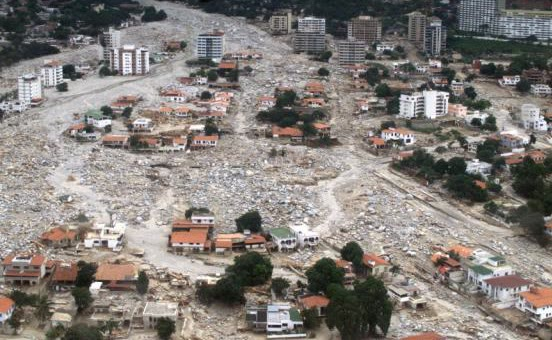
\includegraphics[width=0.62\linewidth]{images/book4/b2-28-caraballeda-debris-flow.jpg}
\par\smallskip{\small Puinstroomafzettingen op de puinwaaier van Caraballeda, aan de kust van Venezuela,
na de storm van december 1999: de stromen verlieten de hoofdgeul en begroeven de stad onder
rotsblokken. Foto Lawson Smith, U.S. Army Corps of Engineers (publiek domein).}
\end{omfigure}
% ledger: photo:b2-28-caraballeda, vargas:caraballeda

\section{Tsunami's}\label{sec:b2:geological-hazards:tsunamis}

Een tsunami die door het plotselinge opheffen van de zeebodem ontstaat, heeft een golflengte van tientallen tot honderden
kilometers, veel meer dan de diepte van de oceaan. Het is een lange golf, en de snelheid ervan hangt alleen
af van de diepte.

\begin{proposition}[Lange golven]\label{prop:b2:geological-hazards:long-waves}
Een zwaartekrachtgolf aan het oppervlak waarvan de golflengte veel groter is dan de waterdiepte $h$, plant zich voort met
$c = \sqrt{gh}$, wat de golflengte ook is. Waar ze langzaam ondieper water in gaat zonder
te reflecteren of te breken, groeit haar amplitude $A$ als $h^{-1/4}$.
\end{proposition}

\begin{proof}
De dispersierelatie geeft de fasesnelheid $c = \omega/k = \sqrt{(g/k)\tanh(kh)}$. Voor een lange
golf is $kh = 2\pi h/\lambda \ll 1$ en $\tanh(kh) \approx kh$, dus $c = \sqrt{gh}$, onafhankelijk van
$k$: lange golven vertonen geen dispersie. De energie van de golf per oppervlakte-eenheid zee is $\frac12
\rho g A^2$, en die energie plant zich voort met $c$. Als er geen energie wordt gereflecteerd of verloren gaat, is de flux $\frac12\rho g A^2
c$ door elke doorsnede langs het pad dezelfde: $A^2 \sqrt{h}$ is constant, en $A \propto
h^{-1/4}$.
\end{proof}

Boven \qty{4000}{m} water plant een tsunami zich voort met \qty{198}{m.s^{-1}}, \qty{713}{km/h}; boven
\qty{5000}{m} met \qty{797}{km/h}, de ``meer dan 800 km/h'' die de waarschuwingsdiensten noemen. Dicht bij de
kust, in \qty{10}{m} water, vertraagt de tsunami tot \qty{36}{km/h}; het front wordt ingehaald door het water
erachter, de golf wordt korter en steiler, en haar hoogte groeit.
% ledger: nws:tsunami-speed

\begin{definition}[Oploophoogte van een tsunami]\label{def:b2:geological-hazards:tsunami}
De \emph{oploophoogte}\index{oploophoogte} van een tsunami op een punt van de kust is de hoogte, boven het
zeeniveau op dat moment, van de hoogste grond die het water daar landinwaarts bereikt. De horizontale
afstand van de kustlijn tot dat punt is de inundatieafstand.
\end{definition}

Meetploegen meten de \omterm{def:b2:geological-hazards:tsunami}{oploophoogtes} na elke tsunami af aan watermerken, aanspoelsellijnen en schade. De
wereldwijde tsunamidatabank bevat \num{2177} oploopwaarnemingen voor de tsunami in de Indische Oceaan van
26 december 2004, veroorzaakt door een aardbeving van magnitude 9.1 voor de kust van Sumatra, met een maximale waterhoogte van
\qty{50.9}{m}, en \num{6429} voor de tsunami van 11 maart 2011 voor de kust van Honshu, eveneens van magnitude 9.1,
met een maximum van \qty{39.3}{m}. De twee kostten \num{227899} en \num{18423} mensen het leven. In Banda Aceh
reikte het water tot halverwege de eerste verdieping van de moskee hieronder.
% ledger: ncei:tsu-2004, ncei:tsu-2011, usgs:aceh-mosque

\begin{omfigure}
\centering
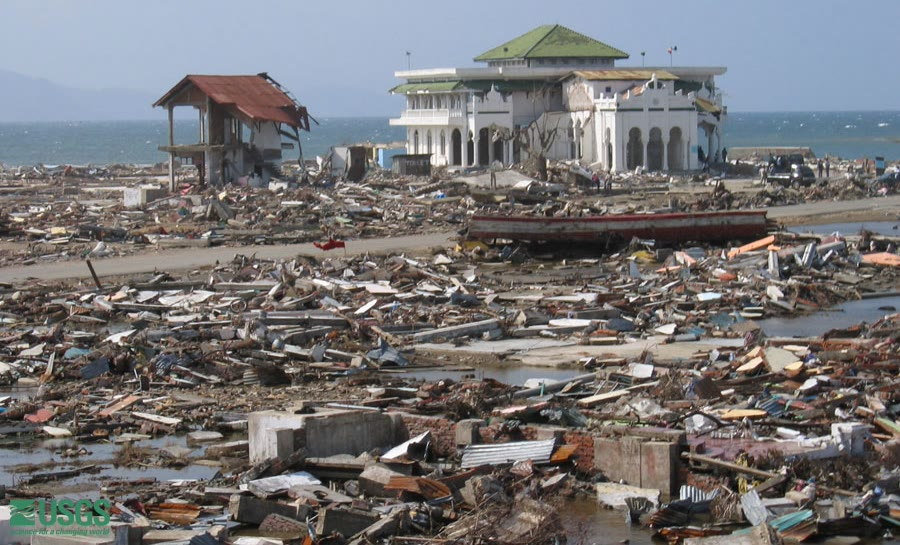
\includegraphics[width=0.62\linewidth]{images/book4/b2-28-aceh-mosque-tsunami.jpg}
\par\smallskip{\small Banda Aceh, Sumatra, op 21 januari 2005, na de tsunami van 26 december
2004: een moskee staat overeind te midden van het puin van de gebouwen eromheen. Foto U.S. Geological
Survey (publiek domein).}
\end{omfigure}
% ledger: photo:b2-28-aceh

\section{Overstromingen}\label{sec:b2:geological-hazards:floods}

\begin{definition}[Hoogwaterfrequentiecurve]\label{def:b2:geological-hazards:flood}
De \emph{hoogwaterfrequentiecurve}\index{hoogwaterfrequentiecurve} van een rivier bij een meetstation is de
curve van de jaarlijkse piekafvoer tegen haar \omterm{def:b2:geological-hazards:return}{terugkeerperiode}, of haar jaarlijkse \omterm{def:b2:geological-hazards:poisson}{overschrijdingskans},
opgebouwd uit de reeks jaarlijkse pieken van het station en meestal verlengd met een aangepaste
kansverdeling.
\end{definition}

De rangformule van de schoolboeken plaatst de punten van de curve. Daar is een reden voor.

\begin{proposition}[Plotpositie van Weibull]\label{prop:b2:geological-hazards:weibull}
Laat $n$ jaarlijkse pieken onafhankelijk zijn en uit dezelfde continue verdeling getrokken, en zij
$G(x)$ de kans dat de piek van een jaar $x$ overschrijdt. De piek met rang $m$, geteld vanaf de
grootste, heeft een verwachte \omterm{def:b2:geological-hazards:poisson}{overschrijdingskans} $m/(n + 1)$, zodat hij wordt uitgezet bij $T = (n +
1)/m$.
\end{proposition}

\begin{proof}
$U = G(X)$ is uniform op $[0, 1]$ voor een continue verdeling, en $G$ is dalend, dus de
$m$-de grootste piek komt overeen met de $m$-de kleinste van $n$ onafhankelijke uniforme variabelen,
$U_{(m)}$. De dichtheid daarvan is $f(u) = \frac{n!}{(m-1)!\,(n-m)!}u^{m-1}(1-u)^{n-m}$: één van de $n$ waarden
bij $u$, $m - 1$ eronder en $n - m$ erboven. Met de bèta-integraal $\int_0^1 u^{p}(1-u)^{q}\,\mathrm{d}u
= p!\,q!/(p + q + 1)!$ geldt
\begin{equation*}
\mathbb{E}[U_{(m)}] = \frac{n!}{(m-1)!\,(n-m)!}\cdot\frac{m!\,(n-m)!}{(n+1)!} = \frac{m}{n+1}. \qedhere
\end{equation*}
\end{proof}

De grootste piek van een reeks van 30 jaar wordt dus uitgezet bij 31 jaar, en niets in de reeks legt
de 100-jaarsoverstroming vast. Om die te bereiken, past men de pieken aan met een extreemwaardenverdeling, vaak die van Gumbel,
$\Pr(\text{piek} \leq x) = \exp\bigl(-e^{-(x - u)/\alpha}\bigr)$, met als $T$-jaarsoverstroming $x_T = u
- \alpha\ln\bigl(-\ln(1 - 1/T)\bigr)$: een rechte lijn tegen $-\ln(-\ln(1 - 1/T))$, die buiten de reeks
wordt geëxtrapoleerd met een risico dat groeit met de afstand.

\section{Monitoring en vroegtijdige waarschuwing}\label{sec:b2:geological-hazards:warning}

\begin{definition}[Vroegwaarschuwingssysteem]\label{def:b2:geological-hazards:warning}
Een \emph{vroegwaarschuwingssysteem}\index{vroegwaarschuwingssysteem} is een geïntegreerd systeem van
monitoring van gevaren, voorspelling, risicobeoordeling, communicatie en paraatheid dat tijdig
handelen mogelijk maakt vóór een gevaarlijke gebeurtenis. Het verenigt vier elementen: kennis van het risico; detectie,
monitoring en voorspelling van het gevaar; de verspreiding van waarschuwingen; en de paraatheid om
te reageren.
\end{definition}
% ledger: undrr:ews

De natuurkunde bepaalt hoeveel tijd elke waarschuwing kan geven. Seismische golven zijn niet te ontlopen, maar de schadelijke
S-golven lopen met ongeveer \qty{3.2}{km.s^{-1}} door de bovenkorst, tegenover \qty{5.8}{km.s^{-1}} voor
de P-golven: een alarm dat wordt berekend uit de eerste P-golven die dicht bij het epicentrum worden geregistreerd, bereikt een stad
vóór de S-golven, met $d(1/3.2 - 1/5.8) = \qty{0.14}{s}$ per kilometer afstand $d$, min de
tijd voor detectie en berekening. Een stad op \qty{100}{km} wint hoogstens \qty{14}{s}; dicht bij de bron krijgt een
blinde zone niets (\cref{exo:b2:geological-hazards:12}). Een tsunami die \qty{100}{km} zee van
\qty{2000}{m} diep oversteekt, doet daar 12 minuten over; over een oceaan duurt het uren. In 2011 werd de Japanse
waarschuwing ongeveer drie minuten na de aardbeving gegeven, maar op basis van een te laag geschatte magnitude,
omdat de instrumenten verzadigd raakten; ze werd ongeveer 28 minuten later bijgewerkt met gegevens van een GPS-boei op zee.
Drukmeters op de diepzeebodem, die de druk op de zeebodem elke 15 seconden omzetten in een
hoogte van het zeeoppervlak, melden passerende tsunami's nu via satellieten.
% ledger: data:prem, jma:warning, ndbc:dart
% values: 0.1401 s/km, 14.0 s at 100 km; 140 m/s over 2000 m, 11.9 min per 100 km (calc/ch28.py)

\begin{inthefield}[Een helling volgen die beweegt]
Op een helling waarvan bekend is dat ze kruipt, plaatsen monitoringteams instrumenten die de variabelen van de
vergelijking van de oneindige helling meten. Piëzometers in boorgaten registreren de poriëndruk op het glijvlak;
inclinometerbuizen, op opeenvolgende diepten afgelezen, tonen waar de grond buigt en hoe snel;
GNSS-stations en extensometers registreren de beweging van het oppervlak; een regenmeter registreert de aanleiding.
De teams vergelijken de beweging met de regen en de waterdruk, seizoen na seizoen, en zoeken
naar de versnelling die aan het bezwijken voorafgaat.
\end{inthefield}

\section*{Oefeningen}\label{sec:b2:geological-hazards:exercises}

Gegevens voor de oefeningen, tenzij anders vermeld: $g = \qty{9.81}{m.s^{-2}}$; volumegewicht van water
\qty{9.81}{kN.m^{-3}}; de GMPE \eqref{eq:b2:geological-hazards:gmpe} op rots ($G_B = G_C = 0$),
$\sigma = 0.230$; P- en S-snelheden in de bovenkorst 5.8 en \qty{3.2}{km.s^{-1}}. Rond af op drie
beduidende cijfers.
% ledger: bjf93:pga, data:prem

\begin{exercise}[$\star$]\label{exo:b2:geological-hazards:1}
Onder het Poisson-model: (a) hoe groot is de kans op minstens één 100-jaarsoverstroming in 30 jaar?
(b) Hoe groot is de kans dat een eeuw verstrijkt zonder 100-jaarsoverstroming? (c) Bepaal de \omterm{def:b2:geological-hazards:return}{terugkeerperiode}
van de beweging met een kans van \qty{5}{\percent} op overschrijding in 50 jaar.
\end{exercise}

\begin{exercise}[$\star$]\label{exo:b2:geological-hazards:2}
Twee steden lopen kans op sterk schudden. In stad A gebeurt dat met een frequentie van één keer in 200 jaar, en het zou
\qty{2}{\percent} van haar 5000 gebouwen verwoesten; in stad B één keer in 50 jaar, met verwoesting van
\qty{10}{\percent} van haar 800 gebouwen. (a) Bepaal het verwachte aantal verwoeste gebouwen per
jaar in elke stad. (b) Welke stad heeft het grootste risico, hoewel ze de kleinste \omterm{def:b2:geological-hazards:risk}{blootstelling} heeft? (c)
Welke van de drie factoren maakt het verschil?
\end{exercise}

\begin{exercise}[$\star$]\label{exo:b2:geological-hazards:3}
(a) Bepaal de snelheid van een tsunami boven diepten van 4000, 200 en \qty{10}{m}. (b) Hoe lang doet hij erover
om \qty{1500}{km} oceaan van \qty{4000}{m} diep over te steken? (c) Op welke diepte zou hij zich voortplanten met
\qty{800}{km/h}?
\end{exercise}

\begin{exercise}[$\star$]\label{exo:b2:geological-hazards:4}
Een droog, cohesieloos zand met $\varphi' = \ang{33}$ vormt een lange helling. (a) Bepaal de
\omterm{def:b2:geological-hazards:slope}{veiligheidsfactor} bij \ang{25}. (b) Wat is de steilste helling die het kan vormen? (c) De helling raakt verzadigd, met
de grondwaterspiegel aan het oppervlak en een kwelstroming evenwijdig eraan, zodat $r_u = \gamma_w\cos^2\beta/\gamma$
met $\gamma = \qty{20}{kN.m^{-3}}$. Toon aan dat $F = (1 - \gamma_w/\gamma)\tan\varphi'/\tan\beta$ en
bereken de factor bij \ang{25}.
\end{exercise}

\begin{exercise}[$\star\star$]\label{exo:b2:geological-hazards:5}
De wereldwijde catalogus bevat 696 aardbevingen van magnitude minstens 7 in de 50 jaar 1976--2025, en
het gemiddelde interval ertussen is 26.2 dagen. (a) Bepaal hun gemiddelde jaarlijkse frequentie. (b) Hoe groot is onder het
Poisson-model de kans dat er 30 dagen verstrijken zonder een ervan? Vergelijk met de waargenomen
fractie intervallen langer dan 30 dagen, 0.304. (c) Hoe groot is de kans op minstens één in een
gegeven week?
\end{exercise}

\begin{exercise}[$\star\star$]\label{exo:b2:geological-hazards:6}
(a) Bepaal de mediane PGA van een aardbeving van magnitude 6.5 op rots bij $d = 0$, 10, 30 en
\qty{100}{km}. (b) Hoeveel zou die bedragen op \qty{10}{km} op een locatie van klasse C? (c) Tussen welke waarden
ligt de PGA op rots op \qty{10}{km} met een kans van ongeveer \qty{68}{\percent}?
\end{exercise}

\begin{exercise}[$\star\star$]\label{exo:b2:geological-hazards:7}
De jaarlijkse piekafvoeren van een rivier over 12 jaar waren, in \unit{m^3.s^{-1}}: 212, 148, 305, 176, 251, 133, 188,
420, 160, 229, 195, 268. (a) Geef de \omterm{def:b2:geological-hazards:return}{terugkeerperioden} van de vier grootste. (b) Schat de
10-jaarsoverstroming door lineair te interpoleren in $\ln T$ tussen de twee grootste. (c) Waarom kan deze reeks
niets betrouwbaars zeggen over de 100-jaarsoverstroming?
\end{exercise}

\begin{exercise}[$\star\star$]\label{exo:b2:geological-hazards:8}
Bij een onrustige vulkaan schat het observatorium: onrust magmatisch 0.6; uitbarsting indien magmatisch 0.4;
explosief indien uitbarsting 0.5; een \omterm{def:b2:eruptive-styles:pdc}{pyroclastische stroom} die een bepaald dal bereikt indien explosief 0.3. (a) Bepaal
de kans op een \omterm{def:b2:eruptive-styles:pdc}{pyroclastische stroom} in het dal. (b) Bepaal de kans op een uitbarsting, en
op een uitbarsting zonder stroom in het dal. (c) Nieuwe deformatiegegevens verhogen de kans op een
uitbarsting, als de onrust magmatisch is, tot 0.7. Werk (a) bij.
\end{exercise}

\begin{exercise}[$\star\star$]\label{exo:b2:geological-hazards:9}
Een droge bodem met $c' = \qty{8}{kPa}$, $\varphi' = \ang{30}$ en $\gamma = \qty{19}{kN.m^{-3}}$ ligt op
een helling van \ang{35}. (a) Bepaal de dikte $z_c$ waarbij $F = 1$. (b) Bepaal $F$ voor een laag
van \qty{2}{m} dik. (c) Dezelfde laag raakt verzadigd, met de grondwaterspiegel aan het oppervlak en
$r_u = \gamma_w\cos^2\beta/\gamma$. Bepaal $F$.
\end{exercise}

\begin{exercise}[$\star\star\star$]\label{exo:b2:geological-hazards:10}
(a) Toon aan dat het Poisson-model geheugenloos is: de kans op geen gebeurtenis in $[s, s + t]$, gegeven
geen in $[0, s]$, is $e^{-t/T}$, wat $s$ ook is. (b) Een breuk heeft een \omterm{def:b2:geological-hazards:return}{terugkeerperiode} van 475 jaar voor haar
grote aardbevingen en heeft er al 400 jaar geen gehad. Hoe groot is, volgens het model, de kans op één
in de komende 50 jaar? (c) De elastische terugveer uit Boek~3 suggereert dat de kans
in plaats daarvan zou moeten groeien met de tijd sinds de laatste aardbeving. Welke aanname van het Poisson-model
spreekt dat tegen, en waarom houden gevarenkaarten het model aan voor oppervlaktebronnen?
\end{exercise}

\begin{exercise}[$\star\star\star$]\label{exo:b2:geological-hazards:11}
Een tsunami met amplitude \qty{0.5}{m} en periode 20 minuten steekt een oceaan van \qty{4000}{m} diep over. (a)
Bepaal met het energiefluxargument uit de propositie over lange golven de amplitude in \qty{10}{m}
water. (b) Bepaal de golflengte op beide diepten. (c) Geef twee redenen waarom de \omterm{def:b2:geological-hazards:tsunami}{oploophoogte} aan de kust
sterk van deze schatting kan afwijken.
\end{exercise}

\begin{exercise}[$\star\star\star$]\label{exo:b2:geological-hazards:12}
Een \omterm{def:b2:geological-hazards:warning}{vroegwaarschuwingssysteem} voor aardbevingen geeft een alarm 4 seconden nadat de P-golf zijn station
het dichtst bij het epicentrum bereikt, op \qty{10}{km} afstand. Verwaarloos de diepte van de bron. (a) Wanneer wordt het
alarm gegeven na de aardbeving? (b) Hoeveel seconden vóór de S-golf ontvangt een stad op \qty{50}{km}
van het epicentrum het alarm? En een stad op \qty{100}{km}? (c) Bepaal de straal van de blinde zone, waar
de S-golf vóór het alarm aankomt.
\end{exercise}

\begin{problem}[{Weekendprobleem --- Een stad tussen een breuk en een helling}]\label{pb:b2:geological-hazards:1}
Een stad op rots ligt op \qty{10}{km} van een bronzone; voor al haar aardbevingen neemt men
$d = \qty{10}{km}$. Hun herhaling is $\log_{10} N(\geq M) = 4.0 - 1.0\,M$ per jaar voor $M \geq 5$,
afgekapt bij $M_{\max} = 7.5$. Het schudden volgt de GMPE \eqref{eq:b2:geological-hazards:gmpe}
met $\sigma = 0.230$. Boven de stad rust een bodemlaag van \qty{3}{m} dik op een helling van \ang{30},
met $\gamma = \qty{19}{kN.m^{-3}}$, $c' = \qty{4}{kPa}$ en $\varphi' = \ang{34}$; water heeft een
volumegewicht van \qty{9.81}{kN.m^{-3}}. Rond af op drie beduidende cijfers.

\noindent\textbf{Deel I --- Herhaling.}
\begin{enumerate}
  \item Bepaal de jaarlijkse frequenties van aardbevingen van magnitude minstens 5, 6 en 7, zonder rekening
        te houden met de afkapping.
  \item Geef de overeenkomstige \omterm{def:b2:geological-hazards:return}{terugkeerperioden}.
  \item Bepaal met de afkapping de frequentie van aardbevingen boven 7.5, en de frequentie van die tussen 7
        en 7.5.
  \item Bepaal de frequenties van de magnitudeschijven 5--6 en 6--7.
  \item Hoe groot is de kans op minstens één aardbeving van magnitude 6 of meer in 50 jaar?
  \item En van magnitude 7 of meer?
\end{enumerate}

\noindent\textbf{Deel II --- Grondbeweging in de stad.}
\begin{enumerate}[resume]
  \item Bepaal $r$, en de afstandsterm $-0.778\log_{10} r$.
  \item Stel de drie schijven voor door de magnitudes 5.5, 6.5 en 7.25. Bepaal de mediane
        $\log_{10}\mathrm{PGA}$ en de mediane PGA van elke schijf.
  \item Bepaal de PGA die door een magnitude 6.5 met een kans van \qty{16}{\percent} wordt overschreden.
  \item Hoe groot is de kans dat een magnitude 6.5 meer dan \qty{0.3}{g} oplevert?
  \item Wat is de mediane PGA van de grootst mogelijke aardbeving?
\end{enumerate}

\noindent\textbf{Deel III --- De gevarencurve.}
\begin{enumerate}[resume]
  \item Bepaal de jaarlijkse overschrijdingsfrequentie van \qty{0.2}{g}, gesommeerd over de drie schijven.
  \item Hetzelfde voor \qty{0.3}{g}.
  \item Hetzelfde voor \qty{0.4}{g}.
  \item Welke jaarlijkse frequentie komt overeen met \qty{10}{\percent} in 50 jaar?
  \item Tussen welke twee van de drie niveaus valt die frequentie?
  \item Bepaal door lineaire interpolatie in $\ln\lambda$ tegen $\ln a$ de PGA met een
        kans van \qty{10}{\percent} op overschrijding in 50 jaar.
  \item Welke schijven dragen het meest bij aan de frequentie bij \qty{0.3}{g}? Geef commentaar, met het antwoord op
        vraag~11.
\end{enumerate}

\noindent\textbf{Deel IV --- De helling boven de stad.}
\begin{enumerate}[resume]
  \item Bepaal de \omterm{def:b2:geological-hazards:slope}{veiligheidsfactor} van de droge helling.
  \item Bepaal hem wanneer de laag verzadigd is, met de grondwaterspiegel aan het oppervlak ($r_u =
        \gamma_w\cos^2\beta/\gamma$).
  \item Tot welke fractie van de laagdikte kan de grondwaterspiegel stijgen voordat de helling bezwijkt?
  \item In een pseudostatische analyse (aangenomen) voegt het schudden een horizontale kracht $kW$ toe. Bepaal de
        kritieke $k$ van de droge helling, waarbij $F = 1$.
  \item Als $k$ gelijk wordt genomen aan de PGA in eenheden van $g$, welke magnitude levert dan de kritieke waarde als
        mediaan in de stad op? Vergelijk met het antwoord op vraag~17.
  \item Samengevat: wat is de \omterm{def:b2:geological-hazards:psha}{piekgrondversnelling} met een kans van \qty{10}{\percent} om in 50 jaar
        te worden overschreden in de stad?
\end{enumerate}
\end{problem}
